% Provenance (never printed): enseignement scientifique premiere (2019),
% "Le Soleil, notre source d'energie" (power received by latitude and
% season, albedo, the Earth's radiative balance, the small share stored by
% photosynthesis) and the old seconde/premiere S material on the
% atmosphere's energy; see sources/book2/PROVENANCE.md. Every insolation
% value, budget closure and photosynthesis figure is computed in
% figdata/grade-10/energy_budget.py; the budget fluxes are AR6 WG1
% Figure 7.2.
\chapter{地球的能量收支}\label{ch:g10:earth-energy-budget}

一年中白昼最长的那一天，北极点的太阳整日不落。它
全天在天空中以相同高度绕行，
离地平线约 \qty{23}{\degree}。极点上空的大气层顶，一天之内每平方米
接收的阳光比地球上其他任何地方都多——
\qty{13.0}{kWh}，赤道上空则为 \qty{9.5}{kWh}。然而极点周围的海面
整个夏季仍被冰层覆盖。而全年来看，赤道接收的阳光
是极点的两倍半，热带终年温暖。
本章沿阳光的能量走向展开：有多少阳光到达，何处、何时到达；有多少
被直接反射回太空；其余部分如何在空气与地面之间分配，
由热带输送向两极，
最终以红外线形式送回太空——
以及其中有多么微小的一部分，最终被
生物储存下来。
% ledger: earth:TSI, earth:obliquity (daily totals computed in figdata/grade-10/energy_budget.py)

\begin{omfigure}
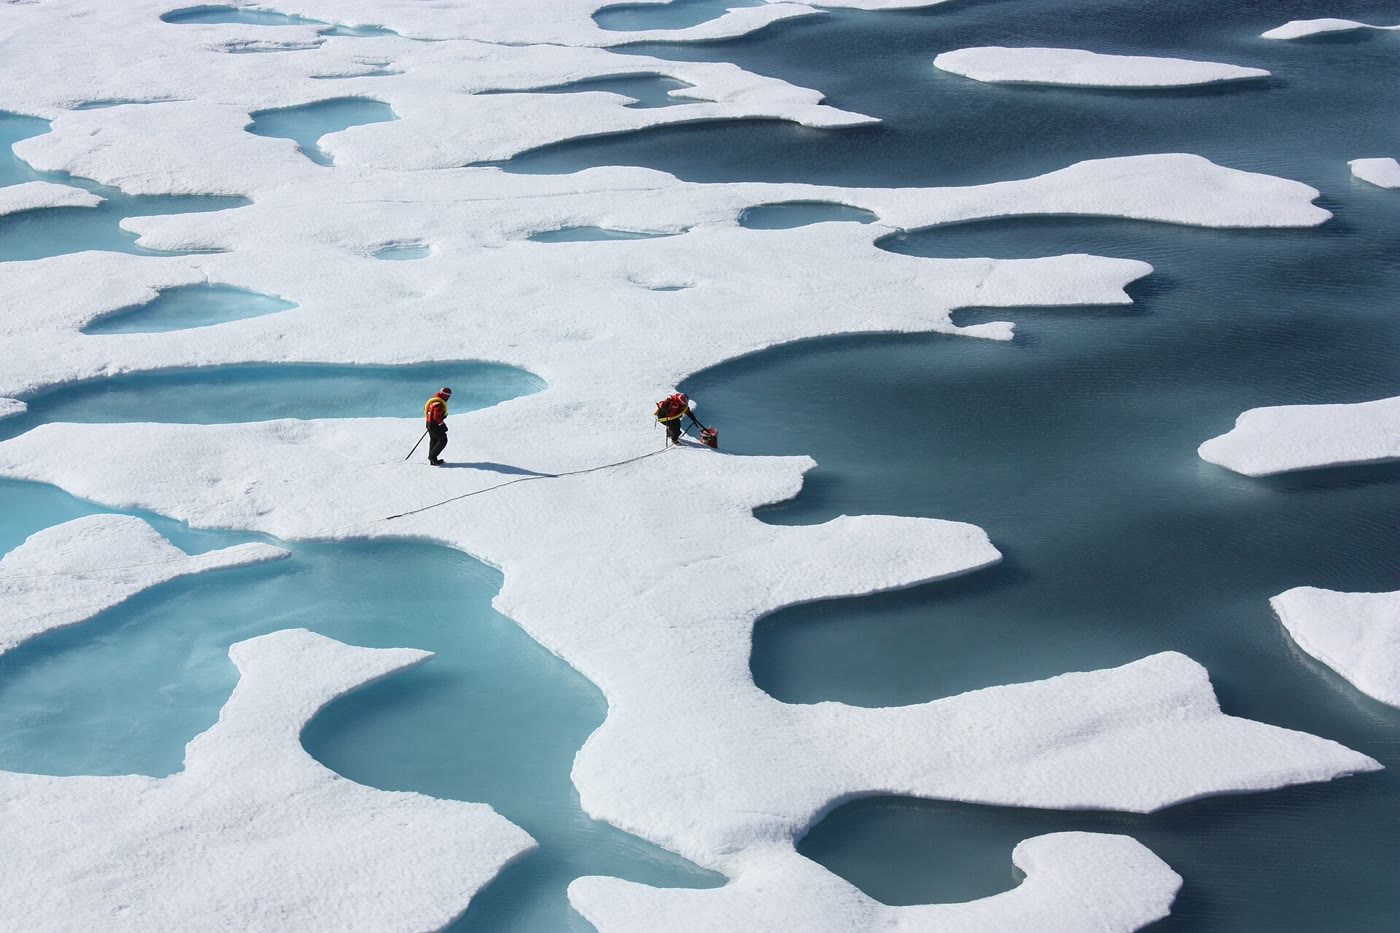
\includegraphics[width=0.78\linewidth]{images/book2/g10-nasa-melt-ponds.jpg}

{\small 七月北冰洋上的海冰，太阳整日不落：
白色的冰面、冰面上的融水池，以及浮冰之间深色的开阔海面：
两位科学家正在取样。照片：NASA 戈达德
太空飞行中心，2011 年，公有领域。}
\end{omfigure}

\begin{recall}
季节源于地轴的倾斜：地轴与轨道平面垂线的夹角为 \qty{23.44}{\degree}，
六月时北半球朝向太阳，太阳在天空中升得更高，
停留的时间也更长（参见物理教材及第 1 册）。
地球距离处的辐照度 $S_0 = \qty{1361}{W/m^2}$，行星的邦德\omterm{def:g10:earth-energy-budget:albedo}{反照率}
及其\omterm{def:g10:habitable-planet:equilibrium-temperature}{平衡温度}，已在
\cref{ch:g10:habitable-planet}中学过。
温室气体吸收地表发射的部分红外线（参见化学教材，
化学教材）。暖空气上升，冷空气下沉，由此使空气
形成对流环流，并驱动全球风系（参见第 1 册，八年级）。
植物、藻类及一些细菌利用光能，由二氧化碳和水制造糖类：
这一过程即光合作用（参见生物教材）。
\end{recall}

\section{接收到的阳光}

从太阳看去，地球是一个圆盘。每秒钟，地球截获的是落在一个
半径为 $R$（即地球自身半径）的圆盘上的阳光；但这些光
被分配到整个球面上，其中一半处于黑夜。

\begin{proposition}[太阳常数的四分之一]\label{prop:g10:earth-energy-budget:quarter}
对整个地球表面并对昼夜取平均，到达大气层顶的
阳光功率为
\[
  \frac{S_0}{4} = \frac{1361}{4} \approx \qty{340}{W/m^2}.
\]
\end{proposition}

\begin{proof}
地球截获的是穿过面积为 $\pi R^2$ 的圆盘的阳光，
该圆盘与光线垂直，即功率为 $S_0\,\pi R^2$。这些能量分布在
面积为 $4\pi R^2$ 的球面上，于是得到 $S_0\,\pi R^2/(4\pi R^2) =
S_0/4$，即每平方米的功率。
\end{proof}
% ledger: earth:TSI, ipcc:budget-toa

\begin{omfigure}
\begin{tikzpicture}[font=\small, >={Stealth[length=2mm]}]
  \foreach \y in {-1.2,-0.8,...,1.21}
    \draw[->, omProp!80!black] (-3.4,\y) -- (-1.75,\y);
  \node[anchor=south, font=\footnotesize, align=center] at (-2.6,1.35) {阳光，\\$S_0$ 每 m$^2$};
  \draw[fill=omProp!15, draw=omProp!80!black] (-1.6,0) ellipse (0.18 and 1.3);
  \node[anchor=north, font=\footnotesize, align=center] at (-1.6,-1.4) {圆盘 \\$\pi R^2$};
  \shade[ball color=omDef!35] (1.2,0) circle (1.3);
  \fill[black, opacity=0.35] (1.2,1.3) arc (90:-90:1.3) arc (-90:90:0.35 and 1.3);
  \draw[omDef!80!black] (1.2,0) circle (1.3);
  \draw[dashed, black!50] (1.2,-1.3) arc (-90:90:0.35 and 1.3);
  \draw[<->] (1.2,0) -- node[above, font=\footnotesize] {$R$} (2.5,0);
  \node[anchor=west, font=\footnotesize, align=left] at (2.8,0.7) {球面 $4\pi R^2$：\\一半在白昼，\\一半在黑夜};
  \node[anchor=west, font=\footnotesize, align=left] at (2.8,-0.75) {平均：\\$S_0\pi R^2/4\pi R^2 = S_0/4$};
\end{tikzpicture}

{\small 地球截获的是落在与自身半径相同的圆盘上的阳光，
但将其分配到面积大四倍的球面上：平均而言，
大气层顶每平方米接收的是
太阳常数的四分之一。}
\end{omfigure}

平均值掩盖了各地之间的巨大差异。一束阳光
斜射到地面时，其覆盖的面积比
正射的光束更大。

\begin{proposition}[水平面上的阳光]\label{prop:g10:earth-energy-budget:height}
太阳位于地平线以上高度 $h$ 处时，大气层顶部一块水平放置的
一平方米面积接收的功率为 $S_0 \sin h$。
\end{proposition}

\begin{proof}
取一束横截面为 \qty{1}{m^2} 的正方形阳光光束，其功率为
$S_0$。它在地面上的投影是一个矩形，一边长 \qty{1}{m}，
另一边沿光线的斜坡方向，长为 $\ell$。在
由该边、光线和光束横截面所构成的直角三角形中，
地面处的角为 $h$，且 $\sin h = 1/\ell$。光束的功率
分布在 $\ell$ 平方米上：$S_0/\ell = S_0 \sin h$，即每
平方米。
\end{proof}

\begin{omfigure}
\begin{tikzpicture}[font=\small, >={Stealth[length=2mm]}]
  \fill[omExo!15] (-0.3,-0.5) rectangle (6.3,0);
  \draw[thick] (-0.3,0) -- (6.3,0);
  \foreach \s in {0,0.3,...,1.21}
    \draw[->, omProp!80!black] ({0.6+\s/sin(35)+3.2*cos(35)},{3.2*sin(35)}) -- ({0.6+\s/sin(35)+0.02*cos(35)},{0.02*sin(35)});
  \draw[omProp!80!black, thick] (0.6,0) -- ({0.6+1.2/sin(35)},0);
  \draw (0.6,0) ++(1.6,0) arc (0:35:1.6);
  \node[font=\footnotesize] at ({0.6+1.85*cos(17)},{1.85*sin(17)}) {$h$};
  \draw[<->] (0.6,-0.25) -- node[below, font=\footnotesize] {$\ell = 1/\sin h$} ({0.6+1.2/sin(35)},-0.25);
  \node[anchor=south west, font=\footnotesize, align=left] at (4.35,1.95) {光束 \\横截面 \\\qty{1}{m^2}};
\end{tikzpicture}

{\small 与地平线成高度角 $h$ 射来的阳光：同一光束
覆盖水平地面 $1/\sin h$ 平方米，因而每平方米
接收的功率为 $S_0 \sin h$。太阳越低，
地面上的阳光就越弱。}
\end{omfigure}

太阳高度一日之内不断变化，昼长则随季节改变；
两者都计入某地所获得的能量。

\begin{definition}[日射量]\label{def:g10:earth-energy-budget:insolation}
某地的\emph{日射量}\index{日射量}，指该地上空大气层顶部
水平放置的每平方米面积所接收到的太阳光功率。
对全天二十四小时取平均，则为\emph{日平均
日射量}；对全年取平均，得\emph{年平均日射量}；两者
均以 \unit{W/m^2} 为单位。
\end{definition}

要算出日平均值，需要知道一日中每一时刻的太阳高度，
这要用到本书之外的数学；下图曲线正是由计算机算出的。
有两种情形较为简单。在
春分时的赤道上，太阳正东升起，正午经过天顶，
十二小时后正西落下。对二十四小时取平均，
所得为 $S_0/\pi \approx \qty{433}{W/m^2}$（在本阶段不加证明地承认）。在北极，
太阳只在天空中以恒定高度绕行，下一例
用到这一点。

\begin{example}[六月的北极]\label{ex:g10:earth-energy-budget:pole}
% ledger: earth:TSI, earth:obliquity (values computed in figdata/grade-10/energy_budget.py)
夏至时，太阳全天都停在北极地平线上方 \qty{23.44}{\degree} 处。
此处日平均\omterm{def:g10:earth-energy-budget:insolation}{日射量}为 $1361
\times \sin 23.44^\circ \approx \qty{541}{W/m^2}$；按二十四小时计，
即 $541 \times 24 \approx \qty{13000}{Wh}$，合每平方米 \qty{13.0}{kWh}。
同一天，赤道接收的日平均值为
\qty{397}{W/m^2}，即每平方米 \qty{9.5}{kWh}：
正午时太阳升得更高，但一天中有十二小时位于地平线以下。
\end{example}

\begin{omfigure}
\begin{tikzpicture}
\begin{axis}[omrecord, width=0.92\linewidth, height=6.4cm, xmin=1, xmax=365,
  ymin=0, ymax=600, ylabel={日平均日射量（\unit{W/m^2}）},
  xtick={1,32,60,91,121,152,182,213,244,274,305,335},
  xticklabels={1,2,3,4,5,6,7,8,9,10,11,12}, xlabel={月份},
  legend style={at={(0.5,1.02)}, anchor=south, legend columns=4, font=\footnotesize, draw=none},
  tick label style={font=\small}, label style={font=\small}]
\addplot[omThm!85!black, thick] table[x=day, y=Q0] {figdata/out/grade-10-energy_budget-daily.dat};
\addlegendentry{赤道}
\addplot[omProp!90!black, thick, densely dashed] table[x=day, y=Q30] {figdata/out/grade-10-energy_budget-daily.dat};
\addlegendentry{北纬\qty{30}{\degree}}
\addplot[omMeth!85!black, thick, dashdotted] table[x=day, y=Q60] {figdata/out/grade-10-energy_budget-daily.dat};
\addlegendentry{北纬\qty{60}{\degree}}
\addplot[omDef!85!black, thick] table[x=day, y=Q90] {figdata/out/grade-10-energy_budget-daily.dat};
\addlegendentry{北极}
\end{axis}
\end{tikzpicture}

{\small 北半球四个纬度处，大气层顶部的日平均\omterm{def:g10:earth-energy-budget:insolation}{日射量}全年变化情况
（假定轨道为圆形，由太阳常数和地轴倾角算得）。
北极有半年得不到日射，
而在夏至前后接收的比其他任何地方都多。}
\end{omfigure}

\begin{remark}[读懂曲线]\label{rem:g10:earth-energy-budget:curves}
赤道的\omterm{def:g10:earth-energy-budget:insolation}{日射量}几乎不变：春分时各有一个较浅的极大值，
此时太阳正午经过天顶。纬度越高，
夏冬之间的起伏越大。
$90^\circ - 23.44^\circ = \qty{66.56}{\degree}$ 以北的地方，冬至时太阳
始终在地平线之下：即极夜。大约自 5 月 10 日
至 7 月底，北极和北纬 \qty{60}{\degree} 处都
比赤道接收到更多的\omterm{def:g10:earth-energy-budget:insolation}{日射量}。
\end{remark}

全年来看，情况有所不同：年平均\omterm{def:g10:earth-energy-budget:insolation}{日射量}
在下文“盈余与亏缺”一节中绘出，自赤道的 \qty{416}{W/m^2} 降至
两极的 \qty{172}{W/m^2}。极地夏季的日照
不足以弥补漫长的极夜和低矮的太阳。

\begin{remark}[日地距离并不造成四季]\label{rem:g10:earth-energy-budget:distance}
% ledger: earth:peri, earth:aph, nasa:earth-perihelion-longitude (ratios computed)
地球轨道并非正圆：它与太阳的距离在
\num{147.1} 与 1.521 亿千米之间变化，变化幅度约为
\qty{3}{\percent}，因此\omterm{def:g10:earth-energy-budget:insolation}{日射量}约变化 \qty{7}{\percent}。
地球在 1 月初离太阳最近，正值北半球
冬季。上图曲线忽略了这一微小变化；四季来自
地轴的倾斜，两个半球的季节恰好相反。
\end{remark}

\section{反照率}

到达地球的阳光中，有一部分从不用来加热任何东西：云、空气、
雪和海洋把它反射回太空。

\begin{definition}[反照率]\label{def:g10:earth-energy-budget:albedo}
某一表面的\emph{反照率}\index{反照率}，是指照射在其上的阳光中被它反射的
比例，是介于 0（光全部被吸收）
与 1（光全部被反射）之间的数。邦德反照率（见\cref{ch:g10:habitable-planet}）
即整个行星的反照率。
\end{definition}

\begin{omfigure}
\begin{tikzpicture}[font=\small, x=9cm, y=0.55cm]
  \foreach \lab/\lo/\hi/\n in {新雪/0.80/0.90/8, 海冰/0.50/0.70/7,
      沙漠沙地/0.40/0.40/6, 地球整体/0.30/0.30/5, 绿草地/0.25/0.25/4,
      裸土/0.17/0.17/3, 针叶林/0.08/0.15/2, 开阔洋面/0.06/0.06/1,
      新铺沥青/0.04/0.04/0} {
    \fill[omDef!45] (0,\n-0.32) rectangle (\lo,\n+0.32);
    \ifdim\hi pt>\lo pt
      \fill[omDef!18] (\lo,\n-0.32) rectangle (\hi,\n+0.32);
      \draw[omDef!80!black] (\lo,\n-0.32) rectangle (\hi,\n+0.32);
    \fi
    \draw[omDef!80!black] (0,\n-0.32) rectangle (\lo,\n+0.32);
    \node[anchor=east, font=\footnotesize] at (-0.01,\n) {\lab};
  }
  \draw (0,-0.6) -- (1,-0.6);
  \foreach \x in {0,0.2,...,1.01}
    \draw (\x,-0.6) -- (\x,-0.75) node[below, font=\footnotesize] {\pgfmathprintnumber[fixed, precision=1]{\x}};
  \node[font=\footnotesize] at (0.5,-2.0) {反照率};
\end{tikzpicture}

{\small 地球整体及各类表面的典型\omterm{def:g10:earth-energy-budget:albedo}{反照率}；条形中的
浅色部分为常见范围。数据来源：科罗拉多大学博尔德分校，
MOSAiC 考察；美国国家冰雪数据中心。}
\end{omfigure}
% ledger: albedo:surfaces, nsidc:albedo-ice

新雪反射了它所接收的大部分光，而开阔的海洋几乎不反射任何光。
这就是开篇照片中的海冰在极地夏季仍能保持低温的原因：
冰面上的积雪最多可反射十分之九的阳光，
而冰块之间的深色海水吸收了约 94\% 的阳光。
冰融化后，深色海水取代了冰面，吸收更多阳光，
使更多的冰融化：这是一个自我增强的循环，
\cref{ch:g12:climate-change}将其列为气候反馈之一。

\begin{omfigure}
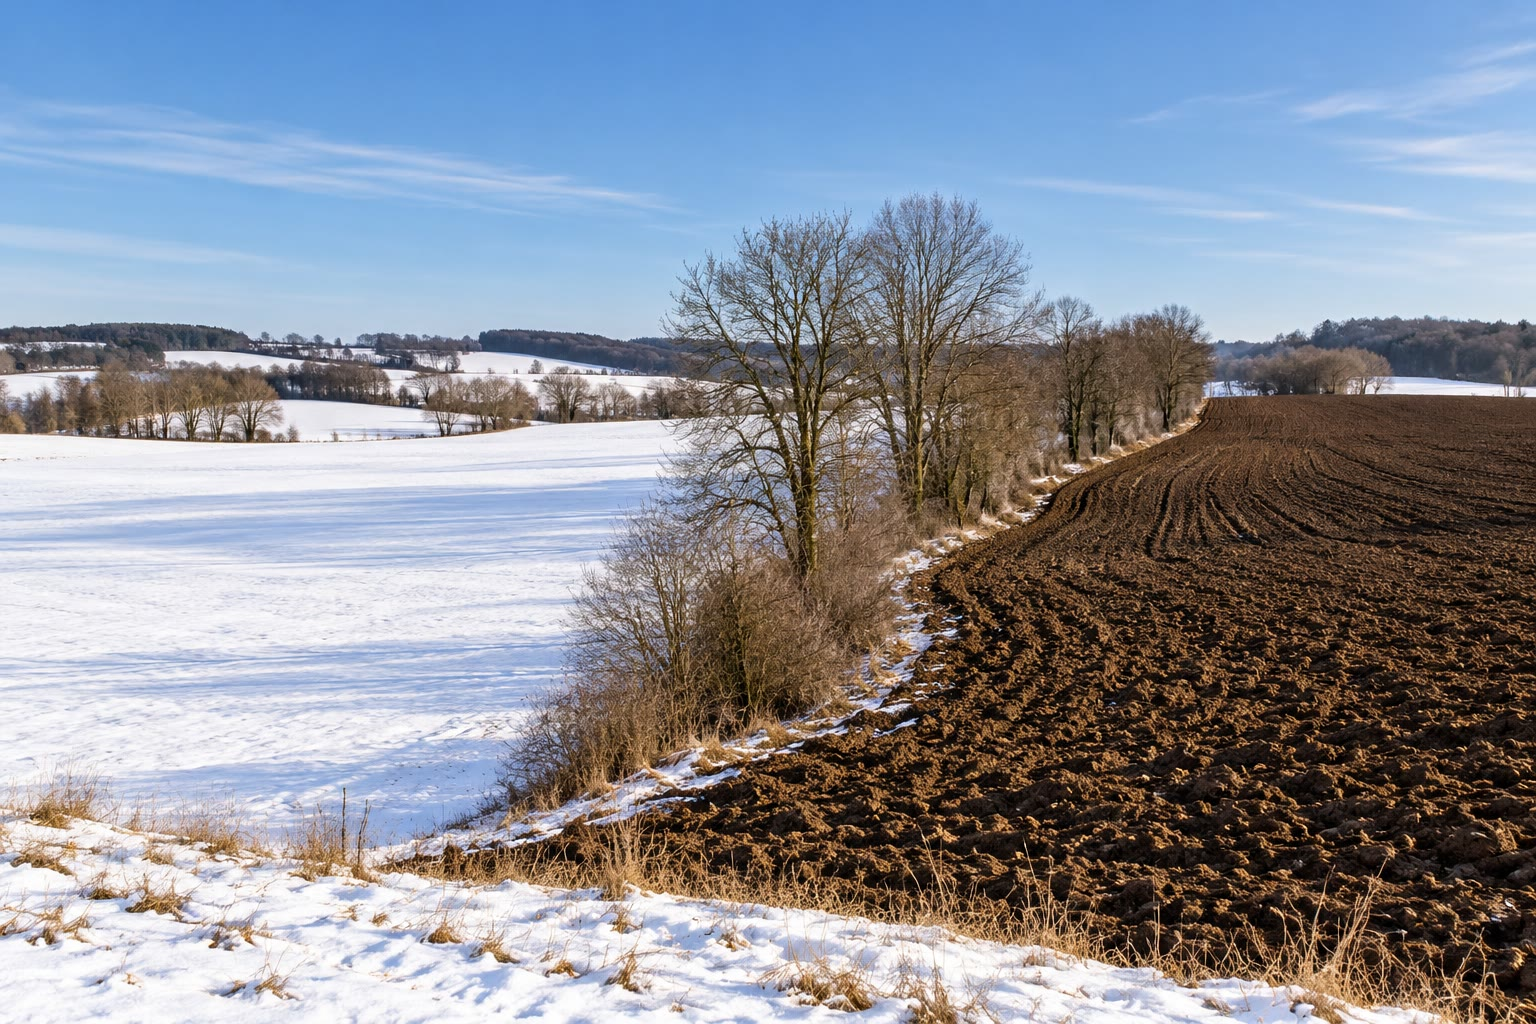
\includegraphics[width=0.7\linewidth]{images/book2/ai/g10-snow-and-ploughed-field.jpg}

{\small 冬日清晨，经过几个晴天后，草地上仍有积雪，
而深色的翻耕农田上积雪已融化，
农田吸收的阳光多得多。}
\end{omfigure}

对整个地球而言，卫星直接测量反射回太空的阳光。平均而言，
反射的 \qty{100}{W/m^2} 占到达的 \qty{340}{W/m^2}，
即\omterm{def:g10:earth-energy-budget:albedo}{反照率}为 $100/340 \approx 0.29$。云是最主要的反射体：
若通过计算去除云，同样的测量仅得出反射量为
\qty{53}{W/m^2}。
% ledger: ipcc:budget-toa, ipcc:budget-clearsky, earth:albedo

\begin{example}[地球吸收的阳光]\label{ex:g10:earth-energy-budget:absorbed}
% ledger: earth:TSI, earth:albedo, earth:Rmean (computed in figdata/grade-10/energy_budget.py)
取邦德\omterm{def:g10:earth-energy-budget:albedo}{反照率}为 0.294，则每平方米平均吸收 $340
\times (1 - 0.294) \approx \qty{240}{W/m^2}$。整个球面的面积为
$4\pi R^2 = 4\pi \times (\qty{6.371e6}{m})^2 \approx \qty{5.10e14}{m^2}$，
故地球吸收的阳光功率为 $240 \times 5.10\times10^{14} \approx \qty{1.22e17}{W}$，
这一功率驱动着风、洋流和
水循环。
\end{example}

\section{全球能量收支}

这 \qty{240}{W/m^2} 的能量去向如何？卫星、地面仪器和船舶的测量，
结合大气模式，
现已给出一致的答案，这一结论基于全球平均及数年平均的结果。
2021 年的科学评估在下图中对此作了总结，
并指出全球平均的各分量现已得到更精确的确定，
包括大气顶层和地表处的数值（\emph{高
置信度}）。
% ledger: ipcc:budget-confidence

\begin{definition}[能量收支]\label{def:g10:earth-energy-budget:energy-budget}
某一系统 --- 整个地球、其表面或其大气 --- 的\emph{能量收支}\index{能量收支}，
是指进入和离开该系统的全部能量的账目，
每一项流量均以地球表面单位面积上的平均功率表示。
当进入的能量与离开的能量相等时，收支称为\emph{平衡}；
否则系统得到或失去能量，
并随之升温或降温。
\end{definition}

地表还会在没有辐射的情况下失去能量：水从海面和叶片上蒸发，
地面也会加热与之接触的空气。

\begin{definition}[潜热；感热]\label{def:g10:earth-energy-budget:latent-heat}
某物质的\emph{潜热}\index{潜热}，是指它在温度不变、状态改变时所吸收的能量 ---
如熔化或蒸发 ---
并在状态反向变化时释放出来。对于
\qty{15}{\degreeCelsius} 下蒸发的水，其潜热约为每千克 \qty{2.47}{MJ}。在\omterm{def:g10:earth-energy-budget:energy-budget}{能量收支}中，
\emph{潜热通量}是指蒸发从地表带走的能量，
以及水汽在空气中凝结成云时所释放的能量。
\emph{感热}\index{感热}通量是指地表传递给与之接触的空气，
使其升温，
并被上升气流向上输送。
\end{definition}
% ledger: nist:water-latent

\begin{omfigure}
\begin{tikzpicture}[font=\footnotesize, >={Stealth[length=2.2mm, width=2mm]}, line width=1.4pt]
  % layers
  \fill[omDef!8] (0,0.5) rectangle (12.8,4.5);
  \fill[omExo!35] (0,0) rectangle (12.8,0.5);
  \draw[thin, black!60] (0,0.5) -- (12.8,0.5);
  \draw[thin, black!60, dashed] (0,4.5) -- (12.8,4.5);
  \node[anchor=east, black!70, align=right] at (-0.1,5.4) {太空};
  \node[anchor=east, black!70, align=right] at (-0.1,4.5) {大气顶层};
  \node[anchor=east, black!70, align=right] at (-0.1,2.5) {大气};
  \node[anchor=east, black!70, align=right] at (-0.1,0.25) {地表};
  \pic[scale=0.7, transform shape] at (4.3,3.0) {puffycloud};
  \pic[scale=0.7, transform shape] at (6.2,3.0) {puffycloud};
  % sunlight
  \draw[->, omProp!90!black] (1.0,6.1) -- (1.0,0.52);
  \draw[->, omProp!90!black] (1.0,3.0) -- (1.6,3.0);
  \node[anchor=west, align=left] at (1.65,3.0) {80 被空气吸收};
  \node[anchor=west] at (1.05,1.3) {185};
  \draw[->, omProp!55] (4.3,3.7) -- (4.3,6.1);
  \node[anchor=east] at (4.25,5.0) {75};
  \draw[->, omProp!55] (5.25,0.52) -- (5.25,6.1);
  \node[anchor=west] at (5.3,1.2) {25};
  % heat
  \draw[->, omMeth!80!black] (6.2,0.52) -- (6.2,2.95);
  \draw[->, omMeth!80!black] (7.8,0.52) -- (7.8,2.0);
  % infrared
  \draw[->, omThm!80!black] (9.2,0.52) -- (9.2,4.0);
  \draw[->, omThm!80!black] (10.7,3.4) -- (10.7,6.1);
  \draw[->, omThm!50] (12.1,4.0) -- (12.1,0.52);
  % words above the top of the atmosphere
  \node[anchor=south, align=center] at (1.0,6.15) {340\\入射};
  \node[anchor=south, align=center] at (4.78,6.15) {100\\反射};
  \node[anchor=south, align=center] at (7.7,5.0) {失衡 \\$+0.7$ 被吸收};
  \node[anchor=south, align=center] at (10.7,6.15) {239 红外 \\射向太空};
  % words below the surface
  \node[anchor=north, align=center] at (1.0,-0.05) {160\\被吸收};
  \node[anchor=north, align=center] at (6.2,-0.05) {82\\潜热};
  \node[anchor=north, align=center] at (7.8,-0.05) {21\\感热};
  \node[anchor=north, align=center] at (9.4,-0.05) {398\\发射};
  \node[anchor=north, align=center] at (12.1,-0.05) {342\\背辐射};
\end{tikzpicture}

{\small 21 世纪初地球的全球平均\omterm{def:g10:earth-energy-budget:energy-budget}{能量收支}，
以 \unit{W/m^2} 计，对整个地表取平均。橙色：
阳光；绿色：由蒸发和暖空气输送的热量；红色：红外线。
在反射的 100 中，25 来自地表，75 来自云层、
大气及其中的尘埃。射向太空的红外线包括地表
辐射中直接穿过大气逸出的部分。数据：IPCC，第六次评估
报告，第一工作组，图~7.2。}
\end{omfigure}
% ledger: ipcc:budget-toa, ipcc:budget-surface

\begin{method}[读懂能量收支图]\label{met:g10:earth-energy-budget:reading}
\begin{enumerate}
  \item 选定系统：整个地球（以大气层顶之上的一条线为界）、
        地表，或大气（二者之间的一层）。
  \item 列出进入该系统的箭头并求和；列出离开该系统的箭头
        并求和。
  \item 比较两个和。若二者在数值取整的误差范围内相等，
        则该系统处于平衡；二者之差即为该系统每秒每平方米
        的得失量（增加或减少）。
\end{enumerate}
\end{method}

\begin{proposition}[收支平衡]\label{prop:g10:earth-energy-budget:balance}
在数据取整的误差范围内，图中所示的收支对整个地球、
地表和大气均达到平衡，
除地球吸收而未再放出的微小盈余之外，其值
约为 \qty{0.7}{W/m^2}。
\end{proposition}

\begin{proof}
\emph{整个地球：}输入 340；输出 $100 + 239 = 339$。\emph{地表：}输入，
$160 + 342 = 502$；输出 $82 + 21 + 398 = 501$。两种情形下的盈余
约为 1，即 0.7 取整后的失衡量。\emph{大气：}记 $W$ 为
地表红外辐射中穿过大气射向太空的部分。大气
接收 $80 + 82 + 21 + (398 - W) = 581 - W$，向下放出 $342$，
向上放出 $239 - W$，合计 $581 - W$：收支平衡，与 $W$ 的取值无关。
\end{proof}
% ledger: ipcc:budget-toa, ipcc:budget-surface (closures checked in figdata/grade-10/energy_budget.py)

图中还显示了正在起作用的温室效应。地表从大气
以红外辐射的形式接收 \qty{342}{W/m^2}——超过其所吸收
阳光的两倍，即 \qty{160}{W/m^2}。这正是它能放出 \qty{398}{W/m^2}，
相当于约 \qty{15}{\degreeCelsius} 物体的辐射，而地球只向太空发出
\qty{239}{W/m^2}。物理教材会建立模型，
把这些数值与温度联系起来，本书则直接使用实测的
通量。

\begin{example}[每年一米水层]\label{ex:g10:earth-energy-budget:evaporation}
% ledger: ipcc:budget-surface, nist:water-latent (computed in figdata/grade-10/energy_budget.py)
\omterm{def:g10:earth-energy-budget:latent-heat}{潜热}通量 \qty{82}{W/m^2} 每秒使每平方米蒸发 $82/2.47\times
10^6 \approx \qty{3.3e-5}{kg}$ 的水。一年按
$3.16\times10^7$ 秒计，共约 \qty{1050}{kg}，相当于覆盖全球、厚
\qty{1.05}{m} 厚的水层。大气中一次只能容纳少量水，
因此这些水几乎全部以雨和雪的形式落回地面：\omterm{def:g10:earth-energy-budget:latent-heat}{潜热}
通量与全球年降水量，是同一水循环的
两个侧面。
\end{example}

\begin{remark}[失衡]\label{rem:g10:earth-energy-budget:imbalance}
% ledger: ipcc:budget-toa, ipcc:heating
与每平方米数百瓦的通量相比，\qty{0.7}{W/m^2} 的盈余显得很小，
但在整个地球上，它为 $0.7 \times 5.10\times10^{14} \approx
\qty{3.6e14}{W}$，主要储存在海洋中，使海洋升温。它并非
一个自然常数：近几十年来它已经增大，
如\cref{ch:g12:climate-change}所述。
\end{remark}

\section{盈余与亏损}

收支对整个地球而言是平衡的，但在各纬度并非如此。

\begin{omfigure}
\begin{tikzpicture}
\begin{axis}[omrecord, width=0.86\linewidth, height=5.6cm, xmin=0, xmax=90,
  ymin=0, ymax=450, xlabel={纬度 (\unit{\degree})},
  ylabel={年平均日射量 (\unit{W/m^2})}, xtick={0,15,...,90},
  tick label style={font=\small}, label style={font=\small}]
\addplot[omThm!85!black, thick] table[x=lat, y=Qann] {figdata/out/grade-10-energy_budget-annual.dat};
\addplot[omDef!80!black, dashed, domain=0:90] {340.25};
\node[anchor=south west, font=\footnotesize, omDef!80!black] at (axis cs:2,343) {全球平均，340};
\node[anchor=south west, font=\footnotesize, omThm!85!black] at (axis cs:62,232) {年平均};
\end{axis}
\end{tikzpicture}

{\small 大气层顶的年平均\omterm{def:g10:earth-energy-budget:insolation}{日射量}随纬度的变化
（两个半球相同，由太阳常数和地轴
倾角计算得到）。在赤道至约 \qty{37}{\degree} 之间，
其值超过全球平均值；向极地则低于该值。}
\end{omfigure}

热带吸收的阳光远多于极地地区，其低\omterm{def:g10:earth-energy-budget:albedo}{反照率}
进一步扩大了这一差距。它们射向太空的红外线也更多，
因为它们更温暖，但随纬度的变化要小得多。因此，
赤道附近地区平均吸收的能量比其反射和辐射的多约 \qty{200}{W/m^2}，
而极地附近地区放出的能量比其吸收的多约
\qty{200}{W/m^2}。
% ledger: nasaeo:surplus

\begin{definition}[向极热量输送]\label{def:g10:earth-energy-budget:heat-transport}
\emph{向极热量输送}\index{向极热量输送}是
由大气和海洋的运动从热带向两极输送的能量流，
其大小以穿过某一纬线圈的功率衡量，
单位为拍瓦（\qty{1}{PW} = \qty{e15}{W}）。
\end{definition}

若无此输送，热带将变得更热，两极将变得更冷，直至每个
纬度各自达到收支平衡。大气承担了大部分输送：
暖空气向极地运动、冷空气回流赤道，以及
水蒸气在远离其蒸发处释放\omterm{def:g10:earth-energy-budget:latent-heat}{潜热}。
洋流承担其余部分。根据测量估计，
大气向极输送量的最大值约为 \qty{5.0}{PW}，出现在
北纬 \qty{43}{\degree} 附近，南纬 \qty{40}{\degree} 附近数值相近；海洋
输送量仅在赤道附近多于大气，即
北纬 \qty{0}{\degree} 至 \qty{17}{\degree} 之间，以及北纬 \qty{35}{\degree} 处，
此处总输送量最大，大气承担其中的
\qty{78}{\percent}。总输送量之所以在此最大，是因为 \qty{35}{\degree} 大致位于
盈余转为亏损的分界处：向赤道方向，输送量持续累积
所经各纬度的盈余；向极方向，每个纬度都从中
取用。
% ledger: trenberth:transport

\begin{omfigure}
\begin{tikzpicture}[font=\footnotesize, >={Stealth[length=2mm]}]
  \def\R{2.4}
  \begin{scope}
    \clip (0,0) circle (\R);
    \fill[omThm!22] (-\R,{-\R*sin(35)}) rectangle (\R,{\R*sin(35)});
    \fill[omDef!22] (-\R,{\R*sin(35)}) rectangle (\R,\R);
    \fill[omDef!22] (-\R,-\R) rectangle (\R,{-\R*sin(35)});
  \end{scope}
  \draw[thick] (0,0) circle (\R);
  \draw[black!50] (-\R,0) -- (\R,0);
  \foreach \s in {1,-1} \draw[black!40, dashed] ({-\R*cos(35)},{\s*\R*sin(35)}) -- ({\R*cos(35)},{\s*\R*sin(35)});
  \node at (0,0.45) {盈余};
  \node at (0,1.95) {亏损};
  \node at (0,-1.95) {亏损};
  \node[anchor=west, black!60] at (\R+0.05,0) {赤道};
  \node[anchor=west, black!60] at ({\R*cos(35)+0.05},{\R*sin(35)}) {\qty{35}{\degree} 北};
  \node[anchor=west, black!60] at ({\R*cos(35)+0.05},{-\R*sin(35)}) {\qty{35}{\degree} 南};
  \foreach \s in {1,-1} {
    \draw[->, very thick, omProp!90!black] ({-(\R+0.35)*cos(10)},{\s*(\R+0.35)*sin(10)}) arc ({180-10*\s}:{180-70*\s}:{\R+0.35});
    \draw[->, thick, omMeth!80!black] ({-(\R-0.45)*cos(8)},{\s*(\R-0.45)*sin(8)}) arc ({180-8*\s}:{180-55*\s}:{\R-0.45});
  }
  \node[anchor=east, omProp!90!black, align=right] at (-\R-0.75,1.6) {大气};
  \node[anchor=east, omProp!90!black, align=right] at (-\R-0.75,-1.6) {大气};
  \node[omMeth!80!black] at (-1.25,0.62) {海洋};
  \node[omMeth!80!black] at (-1.25,-0.62) {海洋};
\end{tikzpicture}

{\small 大致在南纬 \qty{35}{\degree} 与北纬 \qty{35}{\degree} 之间，地球
吸收的能量多于其辐射的能量；在这些纬度的极地一侧，
则辐射多于吸收。大气（橙色）与海洋（绿色）
将盈余输送向两极。示意图：箭头宽度
并非按比例绘制。}
\end{omfigure}

这种输送是天气的动力。第 1 册中的对流环流和
全球风、在\cref{ch:g10:storms-and-cyclones}中的风暴，以及
在\cref{ch:g10:layered-ocean}中的大洋洋流，都将热量从
太阳给予过多的地方输送到给予过少的地方。

\section{能量去向}

地球吸收的太阳能量，几乎全部最终转化为热量：
它加热地面、海洋和空气，使水蒸发，推动
风和洋流，并以红外线的形式再次散失。仅有极小一部分
走了另一条途径：光合作用将其储存在糖类的化学键中，
并由此进入地球上的所有生物质中。

\begin{example}[光合作用的份额]\label{ex:g10:earth-energy-budget:photosynthesis}
% ledger: field:npp, nist:glucose-combustion, earth:Rmean (computed in figdata/grade-10/energy_budget.py)
陆地植物和海洋中的藻类在满足自身需求后，每年约将
\num{105} 十亿吨碳储存于新生成的生物质中，其中大致
约一半在陆地，一半在海洋：生态学家称之为地球的
净初级生产量。燃烧一摩尔葡萄糖，
\ce{C6H12O6}（其中含六摩尔碳，\qty{72}{g}）释放
\qty{2805}{kJ} 的能量：每克碳约 \qty{38.9}{kJ}。每年储存的能量为
$1.049\times10^{17}\,\unit{g} \times \qty{38.9e3}{J/g} \approx
\qty{4.1e21}{J}$，功率为 $4.1\times10^{21}/3.16\times10^{7} \approx
\qty{1.3e14}{W}$。与地球吸收的 \qty{1.22e17}{W} 太阳光相比，
这一比例约为 \qty{0.1}{\percent}。
\end{example}

\begin{remark}[份额虽小，作用却大]\label{rem:g10:earth-energy-budget:life}
被吸收的太阳能量中，千分之一几乎养活了地球上的所有生命，
而植物和藻类的遗骸经过数亿年埋藏，
形成了煤、石油和天然气（见\cref{ch:g11:fossil-fuel-geology}）。
其余的太阳能量——超过 99.9\%——维持着地球的温暖，
并使其空气、水和天气保持流动。
\end{remark}

\section{练习}

\begin{exercise}[$\star$]\label{exo:g10:earth-energy-budget:1}
给出某地\omterm{def:g10:earth-energy-budget:insolation}{日射量}与某表面\omterm{def:g10:earth-energy-budget:albedo}{反照率}的定义。哪种表面
反射的太阳光比例更大：新雪还是开阔海洋？
\end{exercise}

\begin{exercise}[$\star$]\label{exo:g10:earth-energy-budget:2}
利用本章的\omterm{def:g10:earth-energy-budget:energy-budget}{能量收支}图，以到达大气层顶的
\qty{340}{W/m^2} 为基准，分别求出被反射回太空的
部分、被大气吸收的部分以及
被地表吸收的部分各占的百分比。
\end{exercise}

\begin{exercise}[$\star$]\label{exo:g10:earth-energy-budget:3}
夏季阳光向地面提供 \qty{800}{W/m^2} 的辐射。一平方米
地面覆盖新铺沥青（\omterm{def:g10:earth-energy-budget:albedo}{反照率} 0.04）时吸收的功率，以及
覆盖新雪（\omterm{def:g10:earth-energy-budget:albedo}{反照率} 0.85）时吸收的功率各是多少？
\end{exercise}

\begin{exercise}[$\star$]\label{exo:g10:earth-energy-budget:4}
哪一种方式从地表带走的能量更多：蒸发，还是
加热与地面接触的空气？用两句话描述
海洋蒸发所带走的能量如何到达上空的空气。
\end{exercise}

\begin{exercise}[$\star$]\label{exo:g10:earth-energy-budget:5}
解释为什么十二月北极点的日平均\omterm{def:g10:earth-energy-budget:insolation}{日射量}为零，
并给出十二月冬至日时，此现象出现的纬度界限。
\end{exercise}

\begin{exercise}[$\star\star$]\label{exo:g10:earth-energy-budget:6}
利用\cref{prop:g10:earth-energy-budget:height}，计算大气层顶
处水平放置的一平方米所接收的功率，当太阳高出地平线
\qty{90}{\degree}、\qty{30}{\degree} 和 \qty{10}{\degree} 时分别是多少。
太阳高度角为多少时，这一平方米接收的功率为 $S_0$ 的一半？
\end{exercise}

\begin{exercise}[$\star\star$]\label{exo:g10:earth-energy-budget:7}
按照\cref{met:g10:earth-energy-budget:reading}，检验仅考虑
太阳光时的收支：在到达的 \qty{340}{W/m^2} 中，被反射的
部分、被大气吸收的部分和被地表吸收的部分各是多少？三者之和是否为 340？
另外验证到达地表的太阳光 \qty{185}{W/m^2}，
是否全部在地表被反射或吸收。
\end{exercise}

\begin{exercise}[$\star\star$]\label{exo:g10:earth-energy-budget:8}
已知地球平均半径为 \qty{6371}{km}，计算截获阳光的圆盘面积，
并求其截获的功率，再求球面面积。
由此求出球面每平方米的平均功率。
\end{exercise}

\begin{exercise}[$\star\star$]\label{exo:g10:earth-energy-budget:9}
地球的盈余为 \qty{0.7}{W/m^2}，面积为
\qty{5.10e14}{m^2}。以焦耳为单位，地球在
一年（$3.16\times10^7$ 秒）内获得多少能量？
\end{exercise}

\begin{exercise}[$\star\star$]\label{exo:g10:earth-energy-budget:10}
若通过计算去掉云的影响，地球反射的
\qty{53}{W/m^2}（原为 \qty{100}{W/m^2}），并向太空发出 \qty{267}{W/m^2}
的红外线（原为 \qty{239}{W/m^2}）。云使被吸收的太阳光
和损失的红外线各改变了多少？云总体上使地球
变暖还是变冷？
\end{exercise}

\begin{exercise}[$\star\star$]\label{exo:g10:earth-energy-budget:11}
阅读本章中日平均\omterm{def:g10:earth-energy-budget:insolation}{日射量}的曲线。在哪些月份，
北极的日平均\omterm{def:g10:earth-energy-budget:insolation}{日射量}大于赤道的？为什么赤道的曲线
出现两个极大值，而不是一个？
\end{exercise}

\begin{exercise}[$\star\star\star$]\label{exo:g10:earth-energy-budget:12}
水的蒸发\omterm{def:g10:earth-energy-budget:latent-heat}{潜热}为 \qty{2.47}{MJ/kg}，\omterm{def:g10:earth-energy-budget:latent-heat}{潜热}
通量为 \qty{82}{W/m^2}。计算地球平均每平方米每天蒸发的水层
厚度（以毫米计）及每年的厚度（以米计），
（将一升水均匀铺开在一平方米上，形成一层
\qty{1}{mm} 厚的水层）。
\end{exercise}

\begin{exercise}[$\star\star\star$]\label{exo:g10:earth-energy-budget:13}
在北极，太阳沿天空运行，其高度等于
赤纬 $\delta$，因此该处的日平均\omterm{def:g10:earth-energy-budget:insolation}{日射量}为 $S_0 \sin
\delta$。求北极一日内平均接收的\omterm{def:g10:earth-energy-budget:insolation}{日射量}
与春分时赤道相同，即 $S_0/\pi$。赤纬
满足 $\sin\delta = \sin 23.44^\circ \times \sin\lambda$，其中
角 $\lambda$ 在一年内匀速增加 \qty{360}{\degree}，从三月春分时的
\qty{0}{\degree} 起算（六月夏至时为 \qty{90}{\degree}）。
求北极每年约有多少天，其接收的
平均\omterm{def:g10:earth-energy-budget:insolation}{日射量}超过 $S_0/\pi$？
\end{exercise}

\begin{exercise}[$\star\star\star$]\label{exo:g10:earth-energy-budget:14}
假设夏季有 \qty{1e12}{m^2} 面积的海冰（\omterm{def:g10:earth-energy-budget:albedo}{反照率} 0.6）
融化并被开阔洋面（\omterm{def:g10:earth-energy-budget:albedo}{反照率} 0.06）取代，在地表平均
\qty{300}{W/m^2} 的阳光照射下。计算额外
吸收的功率，并将其与地球上所有光合作用
储存的功率 \qty{1.3e14}{W} 相比较，
并解释为何这种地表置换会自我增强。
\end{exercise}

\begin{exercise}[$\star\star\star$]\label{exo:g10:earth-energy-budget:15}
地球到太阳的距离在近日点为 1.471 亿千米，
远日点为 1.521 亿千米，平均值为
1.496 亿千米，其中 $S_0 = \qty{1361}{W/m^2}$。计算
两个极端位置的太阳辐照度。二者之差接近
\qty{90}{W/m^2}；在北纬 \qty{60}{\degree} 处，日平均\omterm{def:g10:earth-energy-budget:insolation}{日射量}在六月约为
\qty{490}{W/m^2}，十二月约为 \qty{24}{W/m^2}。解释为何
距离不能成为季节变化的原因。
\end{exercise}

\section{问题：追随一束阳光}

\begin{problem}[{周末问题——从到达地球的阳光
到生命所储存的份额}]
\label{pb:g10:earth-energy-budget:1}
% ledger: earth:TSI, earth:Rmean, ipcc:budget-toa, ipcc:budget-surface, ipcc:budget-clearsky, nist:water-latent, field:npp, nist:glucose-combustion (all results computed in figdata/grade-10/energy_budget.py or from the rounded data below)
使用 $S_0 = \qty{1361}{W/m^2}$、地球半径 $R = \qty{6371}{km}$，
$\sigma = \qty{5.67e-8}{W.m^{-2}.K^{-4}}$，一年为 $3.156\times10^7$
秒，\omterm{def:g10:earth-energy-budget:energy-budget}{能量收支}图中的各通量，蒸发\omterm{def:g10:earth-energy-budget:latent-heat}{潜热}
为 \qty{2.47}{MJ/kg}，全球净初级生产量为
每年 \num{104.9} 十亿吨碳，以及一摩尔葡萄糖
燃烧时释放的 \qty{2805}{kJ}（其中碳为 \qty{72.07}{g}）。

\medskip
\noindent\textbf{第一部分——阳光的几何。}
\begin{enumerate}
  \item 计算截获阳光的圆盘面积 $\pi R^2$，单位为
        平方米。
  \item 计算它截获的太阳光功率。
  \item 计算地球表面积 $4\pi R^2$。
  \item 由此求出到达大气层顶
        每平方米的平均功率。
  \item 在春分或秋分日正午，太阳直射赤道，
        在北纬 \qty{60}{\degree} 处，太阳高度角为 \qty{30}{\degree}。
        一平方米水平面在两地各接收多少？
\end{enumerate}

\medskip
\noindent\textbf{第二部分——\omterm{def:g10:earth-energy-budget:albedo}{反照率}。}
\begin{enumerate}[resume]
  \item 由反射的 \qty{100}{W/m^2} 计算地球\omterm{def:g10:earth-energy-budget:albedo}{反照率}。
  \item 计算每平方米吸收的功率，以及整个地球吸收的功率。
  \item 若无云，反射量为 \qty{53}{W/m^2}，此时
        \omterm{def:g10:earth-energy-budget:albedo}{反照率}为多少？云使其提高了几倍？
  \item 计算与第 7 题所吸收功率对应的\omterm{def:g10:habitable-planet:equilibrium-temperature}{平衡温度}，
        （见\cref{ch:g10:habitable-planet}），并与地表
        的 \qty{288}{K} 相比较。
\end{enumerate}

\medskip
\noindent\textbf{第三部分——地表。}
\begin{enumerate}[resume]
  \item 求进入地表的各能量通量之和。
  \item 求离开地表的各能量通量之和，并加以比较。
  \item 地表从空气接收的红外线是地表吸收的
        太阳光的多少倍？这说明了什么？
  \item 计算每平方米一年内蒸发的水的质量，
        以及由此形成的水层厚度。
  \item 计算 \qty{0.7}{W/m^2} 的不平衡量
        在整个地球上的总功率。
\end{enumerate}

\medskip
\noindent\textbf{第四部分——生命的份额。}
\begin{enumerate}[resume]
  \item 计算葡萄糖中每克固定碳所储存的能量。
  \item 计算净初级生产量一年内储存的能量。
  \item 将其换算为功率。
  \item 将其表示为每平方米地表面积上的量。
  \item 与第 14 题的不平衡量进行比较。
  \item 光合作用储存的能量占地球所吸收的
        太阳光（第 7 题）的多大份额？
\end{enumerate}
\end{problem}
